%! Author = itgramic
%! Date = 12.01.24

% Preamble
%\section{Statusbericht}
%\KOMAoptions{paper=A3,paper=landscape,DIV=20}
%\storeareas\landscapevaluesbig
%\subsection{Status Report 1}
%\subsection{Status Report 2}
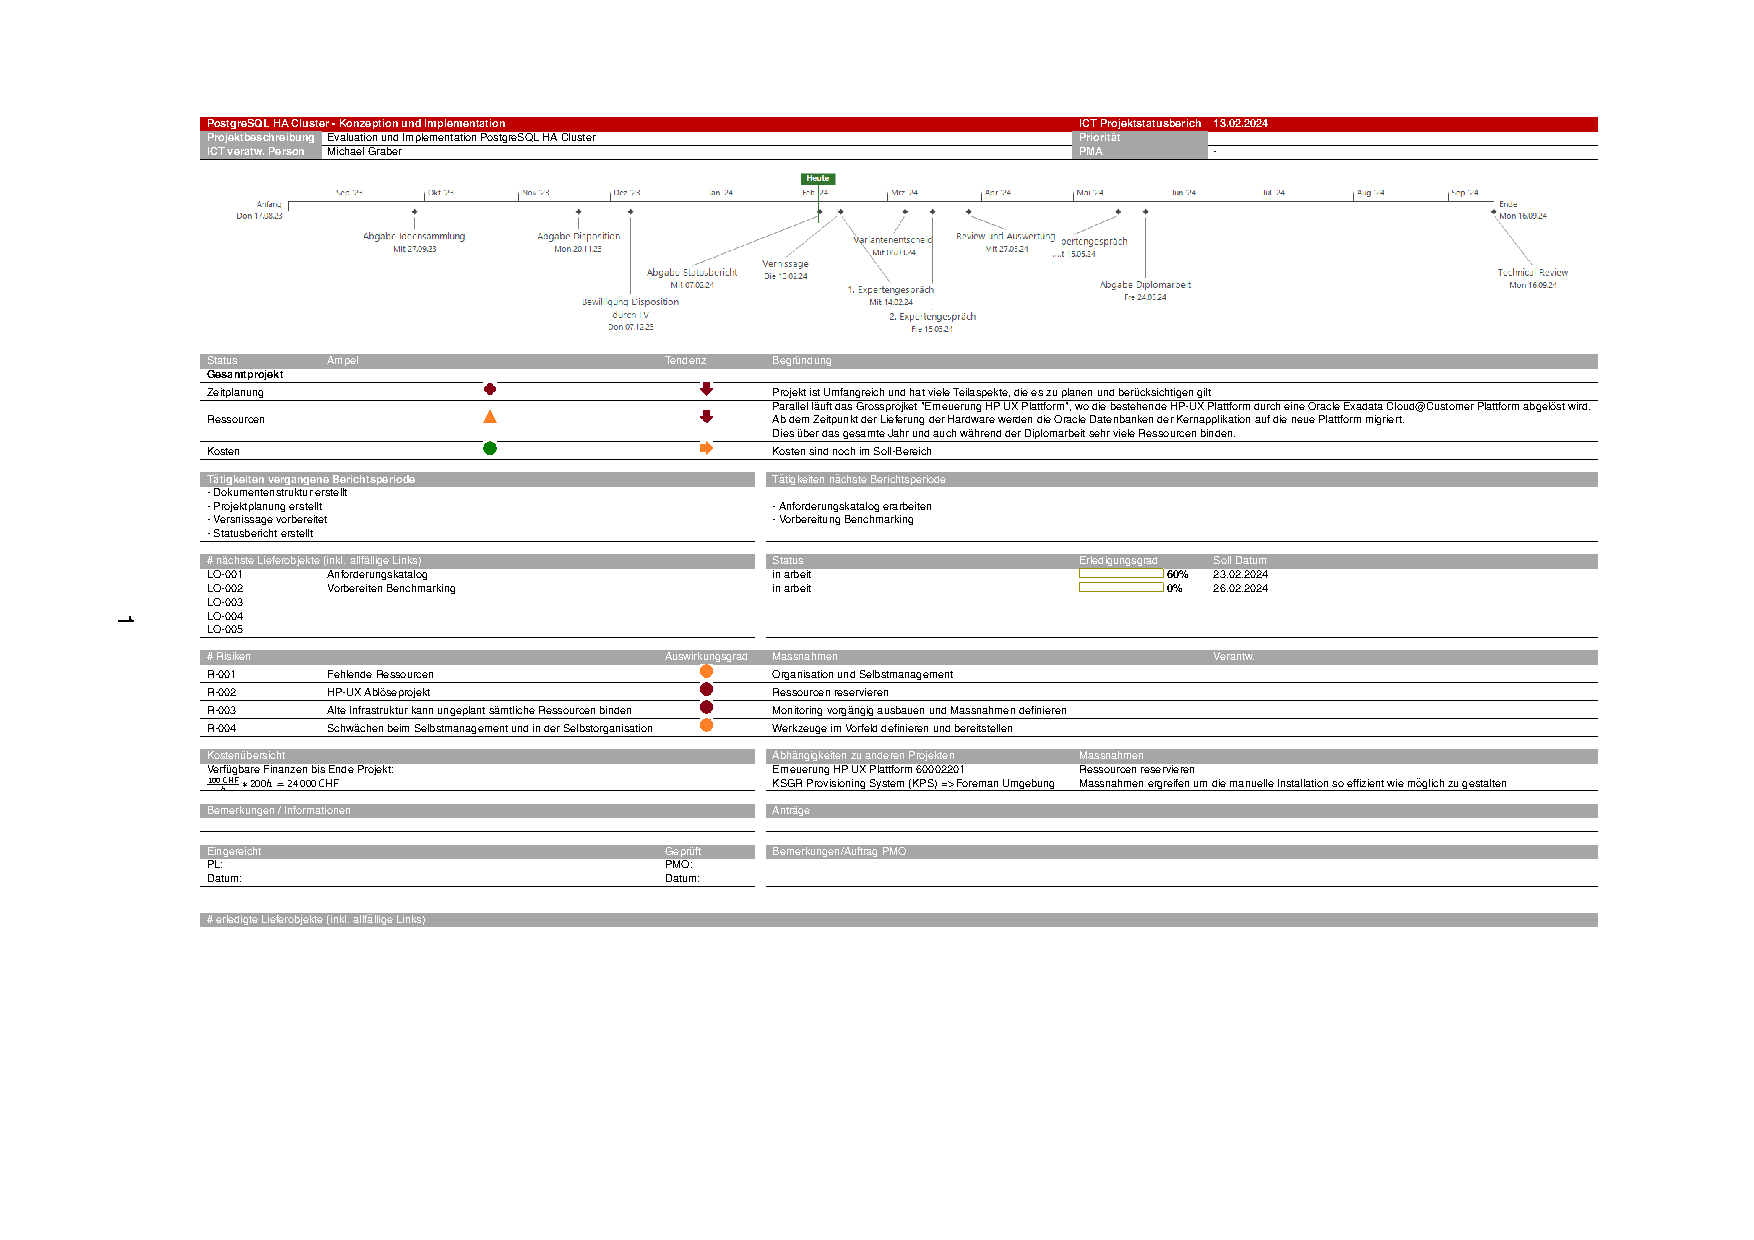
\includepdf[pages=1,pagecommand={\section{Statusbericht}\subsection{Status Report 1}}, fitpaper=true,scale=0.9]{source/projectmanagement_overhead/projectmanagement/status_report/ksgr_statusreport_1.pdf}
\includepdf[pages={2-},fitpaper=true,scale=0.9]{source/projectmanagement_overhead/projectmanagement/status_report/ksgr_statusreport_1.pdf}
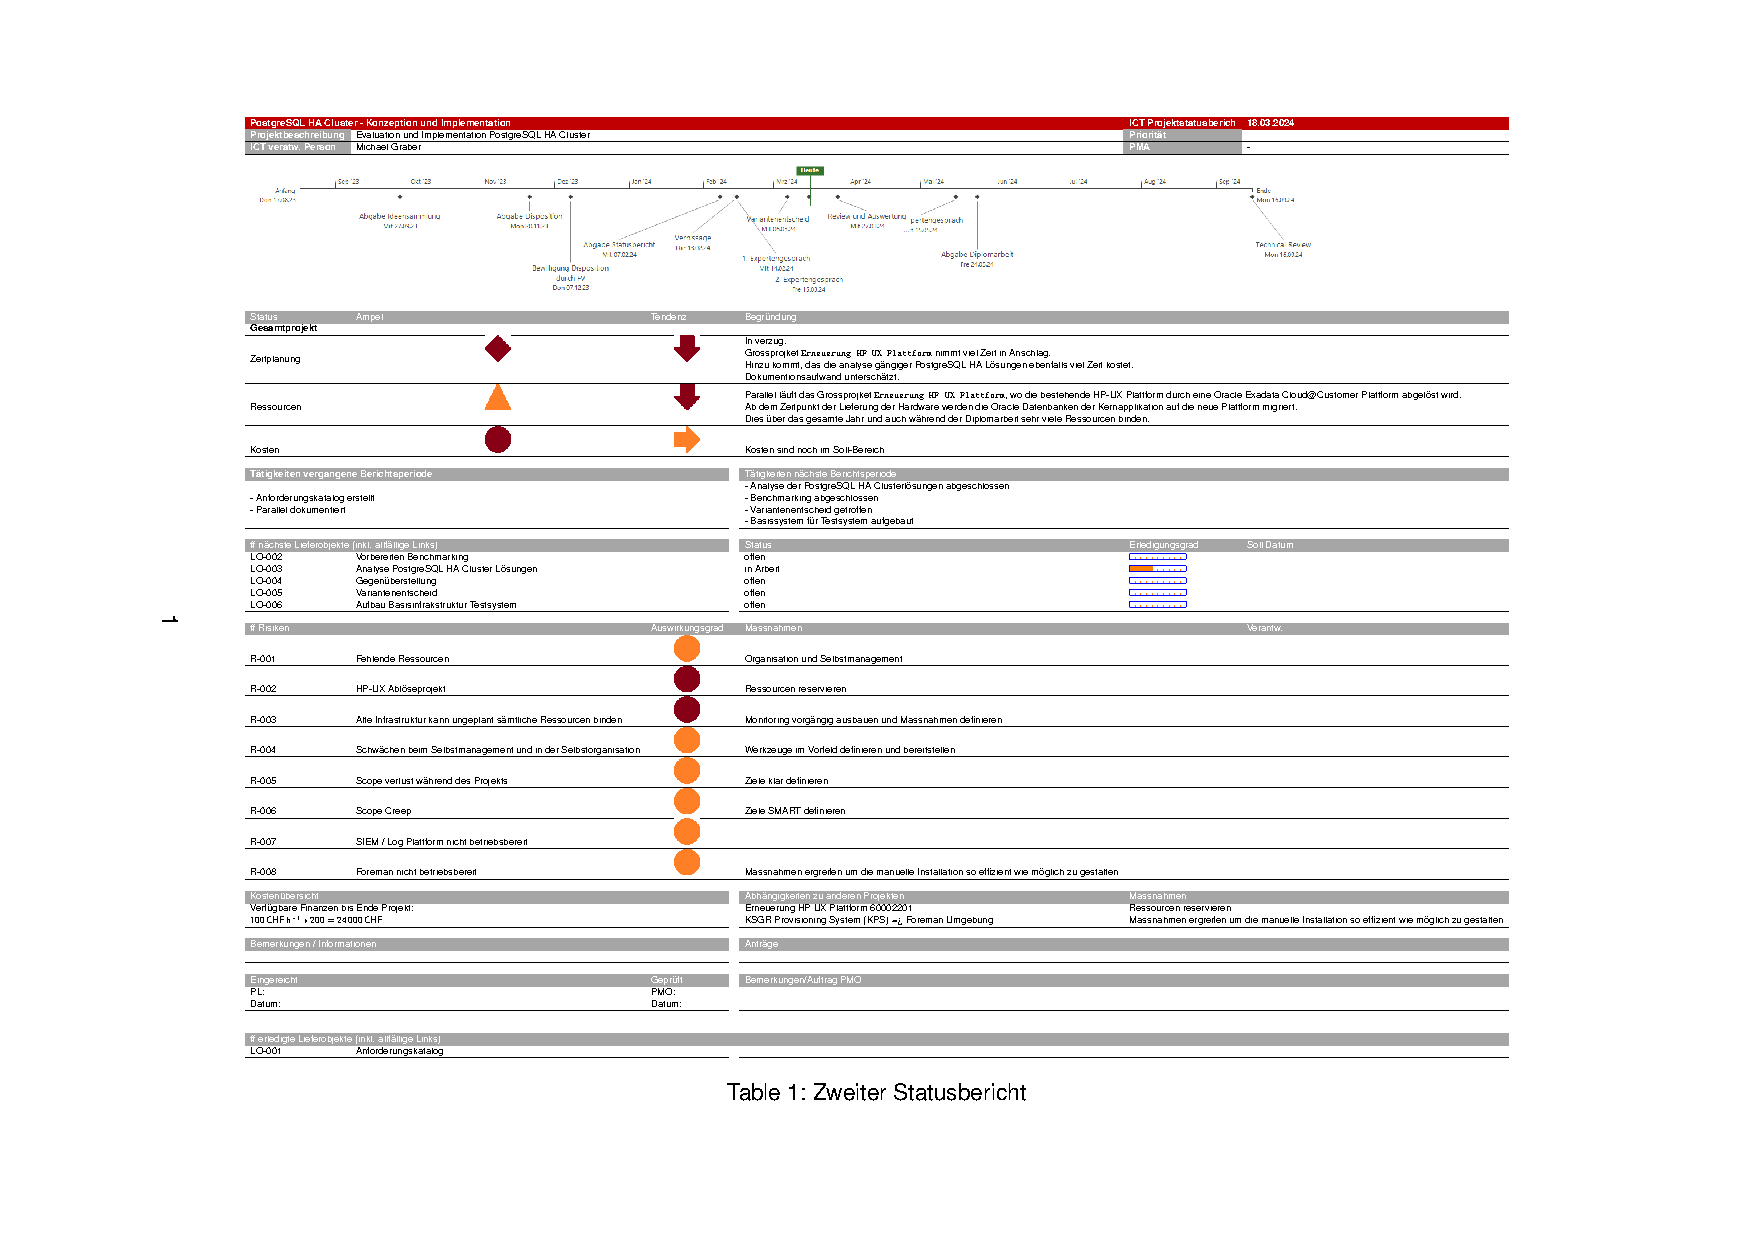
\includepdf[pages=1,pagecommand={\subsection{Status Report 2}}, fitpaper=true,scale=0.9]{source/projectmanagement_overhead/projectmanagement/status_report/ksgr_statusreport_2.pdf}
\includepdf[pages={2-},fitpaper=true,scale=0.9]{source/projectmanagement_overhead/projectmanagement/status_report/ksgr_statusreport_2.pdf}
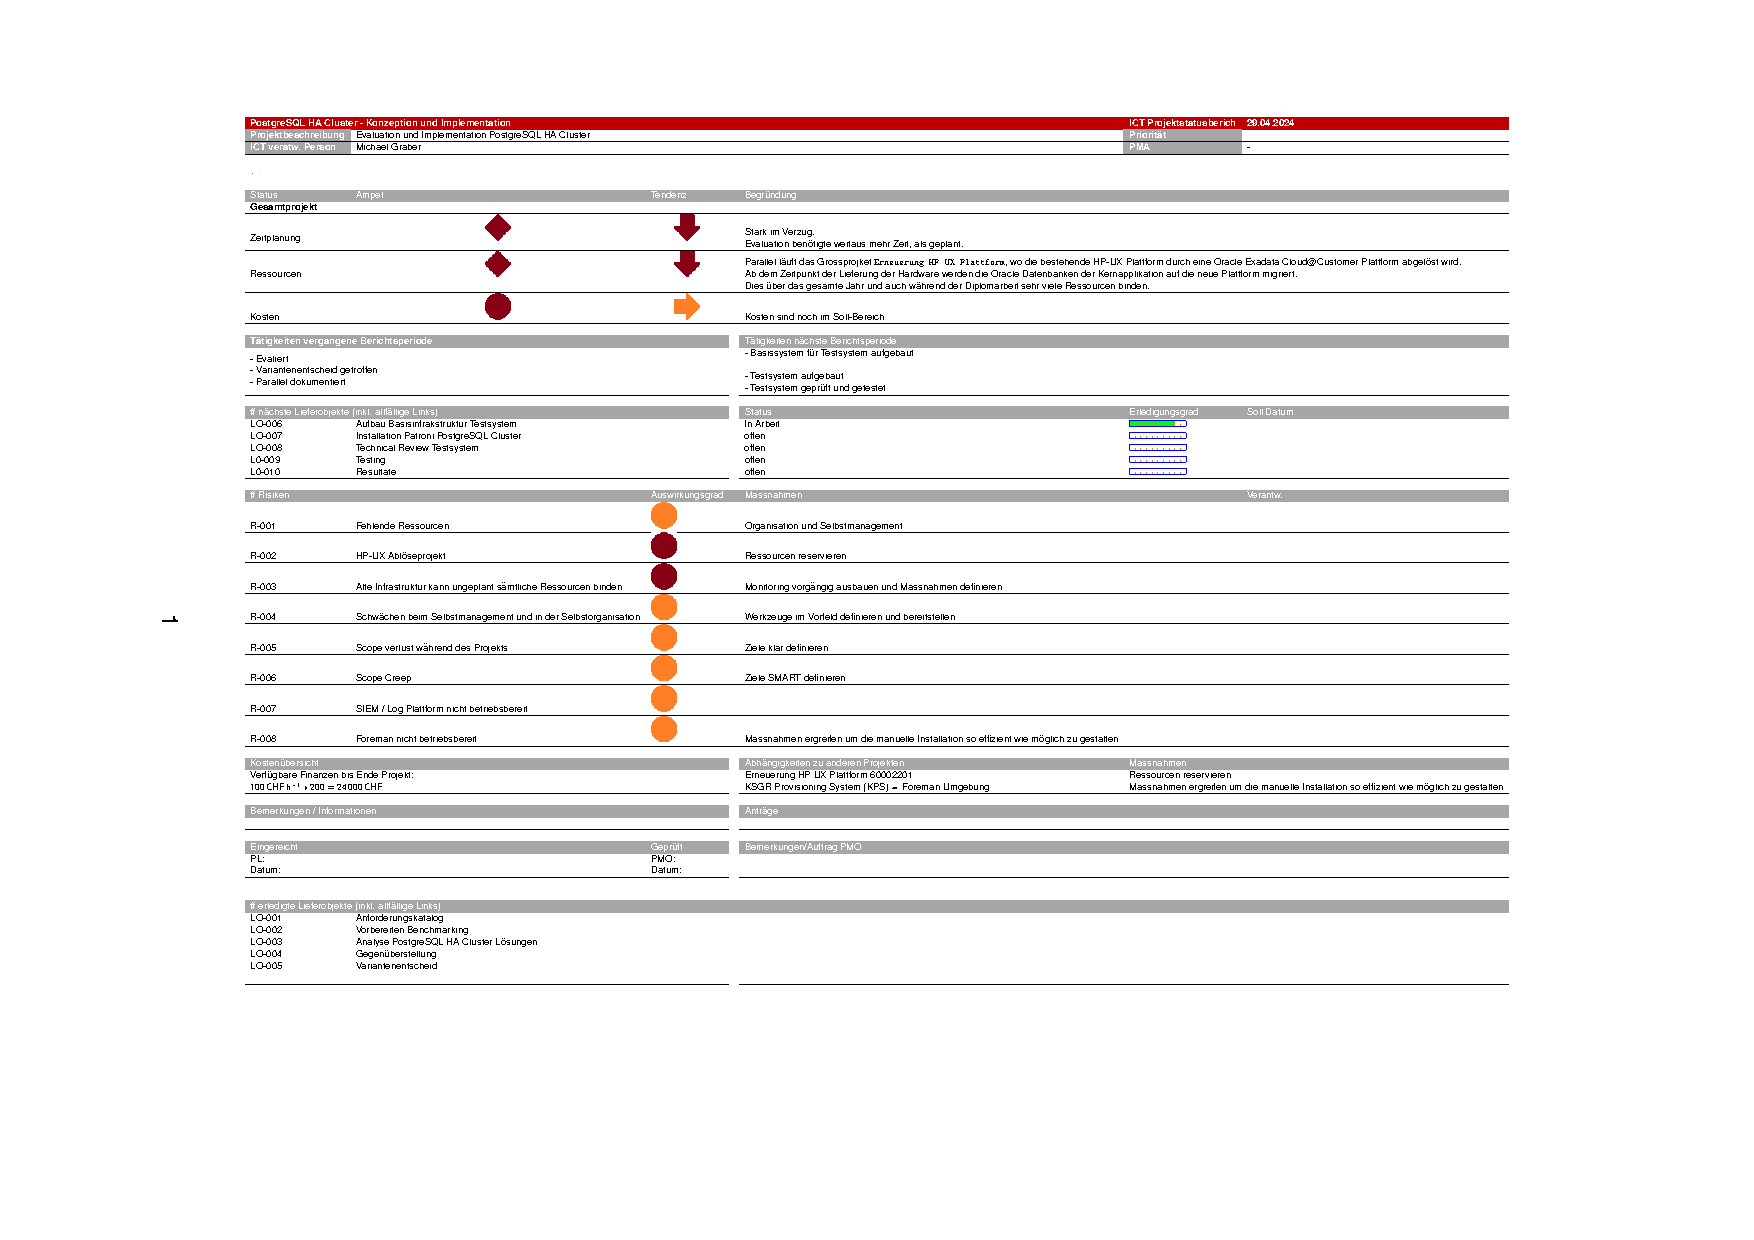
\includepdf[pages=1,pagecommand={\subsection{Status Report 3}}, fitpaper=true,scale=0.9]{source/projectmanagement_overhead/projectmanagement/status_report/ksgr_statusreport_3.pdf}
\includepdf[pages={2-},fitpaper=true,scale=0.9]{source/projectmanagement_overhead/projectmanagement/status_report/ksgr_statusreport_3.pdf}
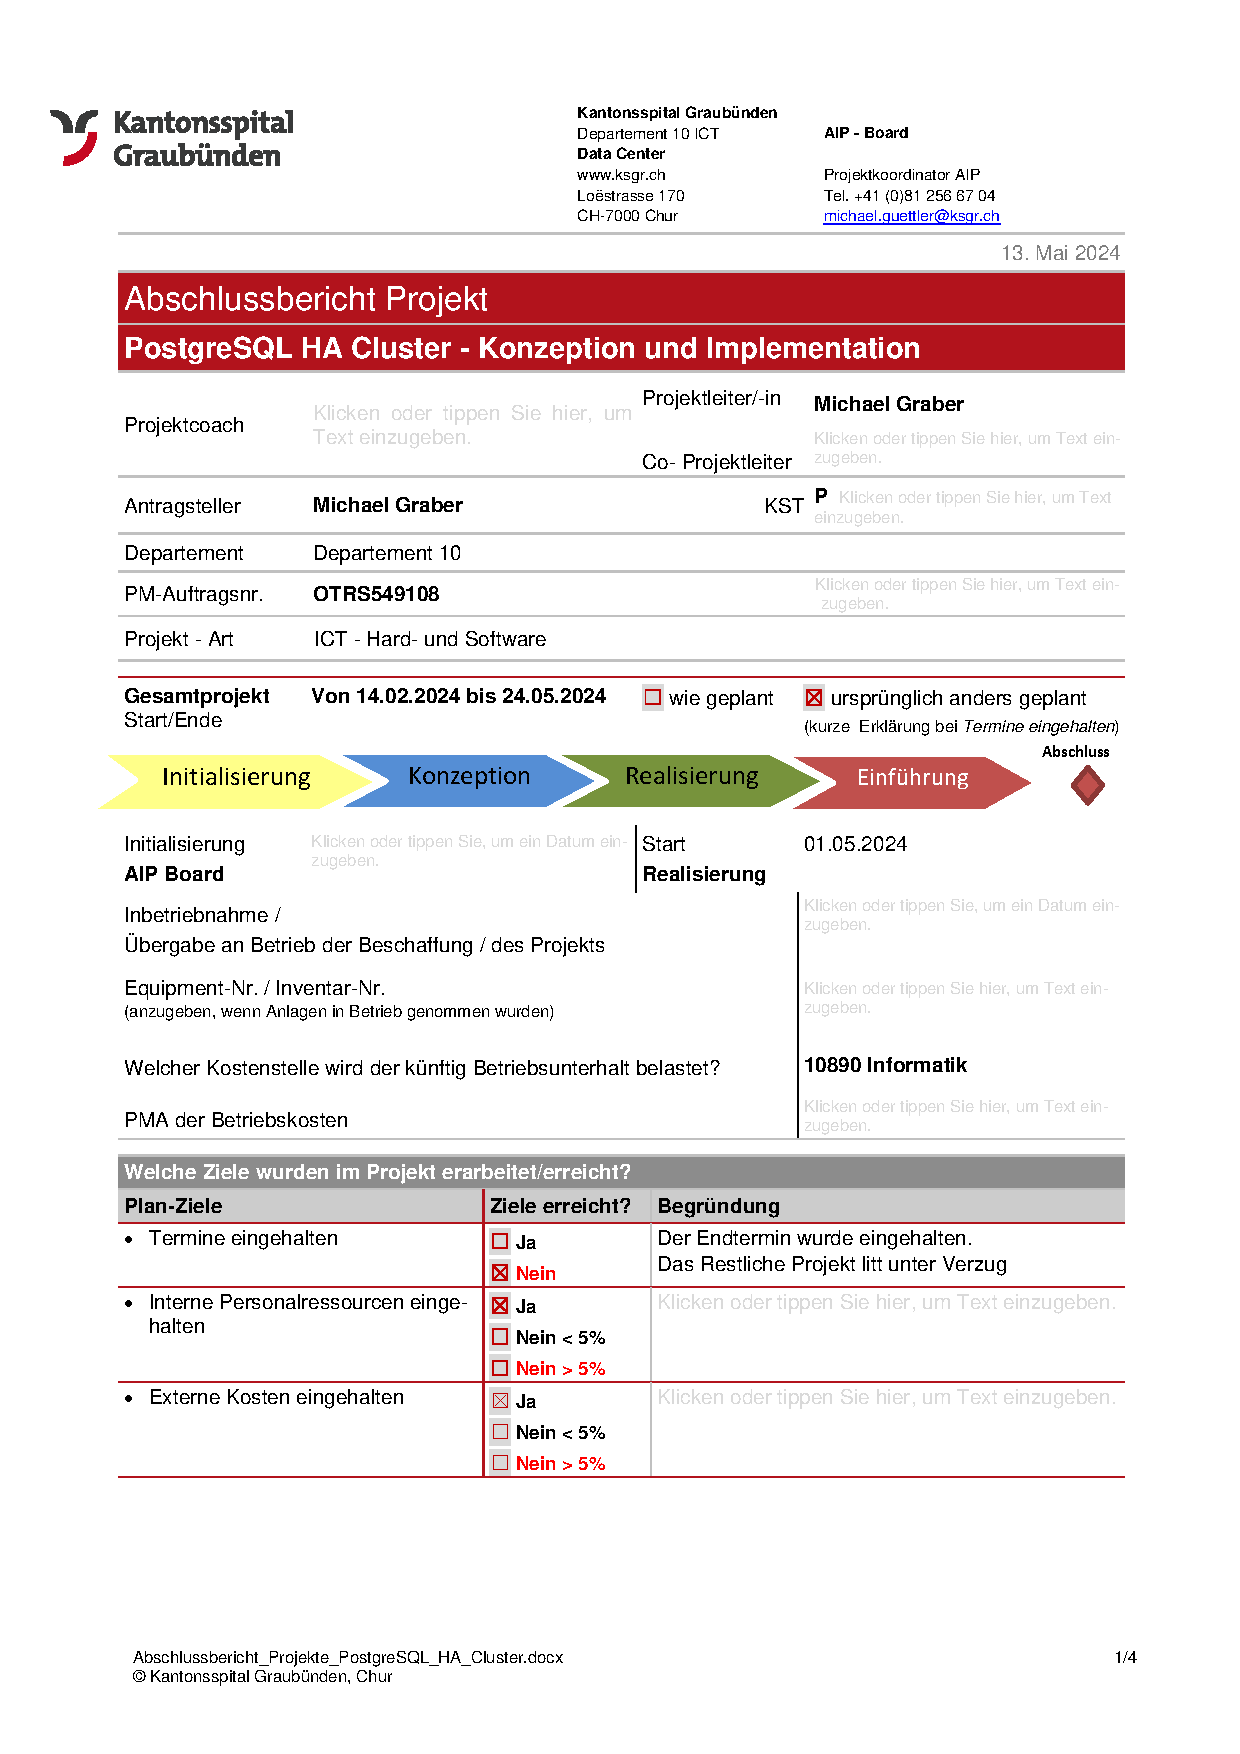
\includepdf[pages=1,pagecommand={\subsection{KSGR Abschlussbericht}}, fitpaper=true,scale=0.9]{source/projectmanagement_overhead/projectmanagement/status_report/Abschlussbericht_Projekte_PostgreSQL_HA_Cluster.pdf}
\includepdf[pages={2-},fitpaper=true,scale=0.9]{source/projectmanagement_overhead/projectmanagement/status_report/Abschlussbericht_Projekte_PostgreSQL_HA_Cluster.pdf}